\documentclass{article}
\usepackage{spconf,amsmath,amssymb,graphicx,booktabs,array,microtype,dblfloatfix,float}
\graphicspath{{figures_icassp/}}
% Automatically generated from outputs/icassp_primary/summary.csv.
\newcommand{\PixelFisherRange}{0.277--0.520}
\newcommand{\CaseSpearmanRange}{0.890--0.966}
\newcommand{\NAURCRange}{0.024--0.092}
\newcommand{\RRRFiftyRange}{19.3--52.1\%}

% Automatically generated from outputs/shared_error_stress/summary.csv.
\newcommand{\StressMaeIncrease}{14.9\%}
\newcommand{\StressTargetIncrease}{28.6\%}
\newcommand{\StressSharedChange}{0.0\%}
\newcommand{\StressCommitteeMaeIncrease}{11.8\%}

\newcommand{\CrossScaleRhoRange}{0.871--0.937}
\newcommand{\CrossScaleNAURCRange}{0.052--0.098}
\newcommand{\CrossScaleRRRRange}{18.8--22.2\%}
\newcommand{\MatchedAdvantageRange}{-0.010--0.014}
\newcommand{\MedianMeanDelta}{-0.001 [-0.008, 0.008]}
\newcommand{\MedianSpreadDelta}{0.011 [-0.007, 0.031]}

\setlength{\textfloatsep}{6pt plus 2pt minus 2pt}
\setlength{\dbltextfloatsep}{6pt plus 2pt minus 2pt}
\setlength{\floatsep}{5pt plus 2pt minus 2pt}
\setlength{\intextsep}{5pt plus 2pt minus 2pt}
\setlength{\tabcolsep}{3.0pt}
\renewcommand{\arraystretch}{0.94}
% Use the reference-only fifth page efficiently without changing margins or font size.
\makeatletter
\let\oldthebibliography\thebibliography
\renewcommand{\thebibliography}[1]{%
  \oldthebibliography{#1}%
  \setlength{\itemsep}{11.8pt plus 0.6pt minus 0.5pt}%
  \setlength{\parsep}{0pt}%
  \setlength{\parskip}{0pt}%
}
\makeatother

\title{TARGET-TO-COMMITTEE DISAGREEMENT FOR MRI SLICE REVIEW:\\
SELECTION, TRANSFER, AND FAILURE BOUNDARIES}
\name{Anonymous Authors}
\address{Anonymous submission}

\begin{document}
\ninept
\maketitle

\begin{abstract}
Cohort-average fidelity cannot identify which MRI interpolation should be reviewed when the missing target is unavailable. We evaluate ground-truth-free ranking from deterministic outputs: a target interpolator is excluded from a heterogeneous committee, and its median absolute target-to-member difference is aggregated over generated foreground voxels. Ground truth is isolated from scoring. Beyond evaluating a fixed score, we register 132 score--mask--pooling candidates and 40 score--committee combinations on IXI $\times4$ and fastMRI-brain $\times2/\times4/\times6$, freeze four finalists, and validate once on 22 eight-fold out-of-fold NingXia examinations at all three factors. The development-selected committee reduces mean nAURC from 0.089 to 0.040, but degrades it from 0.070 to 0.116 on frozen validation. The pre-specified score remains strongest (Spearman 0.901, nAURC 0.070, RRR50 21.8\%). This transfer failure, paired bootstrap analysis, and common-mode error decomposition show that committee selection can overfit cohort difficulty. Disagreement is a selective-review signal, not calibrated uncertainty or a clinical guarantee.
\end{abstract}

\begin{keywords}
MRI interpolation, reliability ranking, selective review, model disagreement, quality control
\end{keywords}

\section{Introduction}
Through-plane interpolation densifies sparse MRI stacks for visualization, registration, and volumetric processing. Modern methods model inter-slice context or adapt restoration transformers \cite{song2024i3net,liang2021swinir,chen2022hat}, yet they are usually compared by cohort-average PSNR, SSIM, or MAE. Such metrics summarize a test set but do not identify an unreliable examination once the missing slice is unobservable.

Model-internal uncertainty methods use stochastic inference, repeated training, heteroscedastic objectives, TTA, posterior reconstruction, or learned error prediction \cite{gal2016dropout,lakshminarayanan2017deepensembles,kendall2017uncertainties,wang2018tta,edupuganti2021uqmri,kuestner2024ensembles,shaw2020heteroscedastic,hu2021predict,zhang2024trainingfree}; no-reference MRI quality assessment instead targets perceptual quality or acquisition artifacts \cite{stepien2022nriqa}. Our setting is different: only deterministic outputs from established interpolators are assumed. Selective prediction supplies the endpoint: retain low-score examinations and refer high-score examinations \cite{elyaniv2010selective,geifman2019selectivenet,ding2020aurc,kompa2021second}. We contribute (1) a self-excluded target-to-committee ranking protocol and common-mode error boundary, (2) a registered candidate funnel with strict development/validation separation, and (3) a multi-factor transfer study showing that development-selected committees need not improve independent-cohort review.

\section{Method}
\subsection{Deployment contract and target isolation}
Let $x$ denote observed sparse-slice context, $y$ the unobserved dense target, and $\hat y_m=f_m(x)$ the output of target interpolator $m$. Available output identities form $\mathcal B$, and the target-specific committee is
\begin{equation}
 \mathcal C_m=\{\hat y_b:b\in\mathcal B,\ b\neq m\}.
 \label{eq:committee}
\end{equation}
The committee may combine neural point reconstructions with deterministic analytical interpolation, but never contains $y$ or $\hat y_m$ itself. Before scoring, outputs must share case identity, affine, orientation, voxel grid, shape, generated-slice pattern, and source-intensity representation. Missing, duplicate, non-finite, or geometrically mismatched files invalidate the profile rather than being silently resampled. Disagreement is meaningful only under this deployment contract.

\begin{figure}[!t]
 \centering
 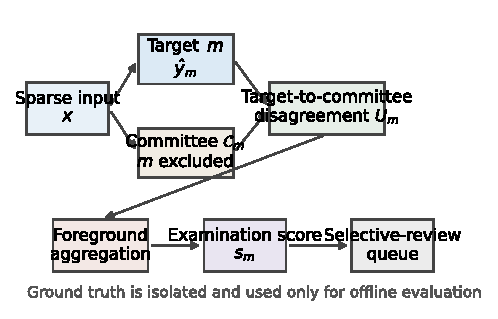
\includegraphics[width=0.98\columnwidth]{figure_framework_outlined.pdf}
 \caption{Target-specific scoring and offline evaluation. The target is excluded from its heterogeneous committee; ground truth is revealed only after scoring.}
 \label{fig:framework}
\end{figure}

\subsection{Target-specific disagreement family}
For generated voxel $i$, the default map is
\begin{equation}
 U_m(i)=\mathop{\mathrm{median}}_{b\in\mathcal C_m}
 |\hat y_m(i)-\hat y_b(i)|.
 \label{eq:score}
\end{equation}
This is a median target-to-committee difference, not statistical median absolute deviation and not posterior variance. Self-exclusion is essential because including $\hat y_m$ creates a structural zero. To separate the protocol from the elementary aggregator, define $d_{mb}(i)=|\hat y_m(i)-\hat y_b(i)|$ and
\begin{equation}
 U_m^g(i)=g\!\left(\{d_{mb}(i):b\in\mathcal C_m\}\right),
 \label{eq:family}
\end{equation}
where $g$ may be the median, mean, maximum, or trimmed mean. Comparators also include distance to the committee mean/median image, target-excluded committee spread, mean/median pairwise disagreement, residuals to linear/cubic interpolation, and gradient- or Laplacian-domain variants. These tests distinguish robust target conditioning from generic set dispersion, analytical departure, and local structural inconsistency. Changing the named target changes every $d_{mb}$ and may change the review order; a single all-output spread map cannot attribute risk to one interpolator.

\subsection{Generated support, masking, and intensity}
For factor $r$, let $\mathcal Z_{\rm obs}^{(r)}$ be the recorded anchor indices and $\mathcal Z_{\rm gen}^{(r)}=\mathcal Z\setminus\mathcal Z_{\rm obs}^{(r)}$. The audited runs begin at anchor $a=0$, hence $\mathcal Z_{\rm obs}^{(r)}=\{z:(z-a)\bmod r=0\}$; define $\mathcal G_r=\{i:i_z\in\mathcal Z_{\rm gen}^{(r)}\}$. Observed anchors are never scored. The default deployment mask and examination score are
\begin{align}
 M_m^{(r)}(i)&=\mathbf1\!\left[|\hat y_m(i)|>0.01\max_{j\in\mathcal G_r}|\hat y_m(j)|\right],\label{eq:mask}\\
 s_m^{(r)}&=\frac{\sum_{i\in\mathcal G_r}M_m^{(r)}(i)U_m(i)}{\sum_{i\in\mathcal G_r}M_m^{(r)}(i)}.
 \label{eq:case}
\end{align}
The formulation is independent of factor; $r$ only determines $\mathcal G_r$. Each factor forms a separate review queue because raw score scales need not be comparable. Foreground aggregation prevents background dominance, although a target mask may omit suppressed tissue. Ground-truth masks are rejected by the deployment path. Predictions share the source-volume intensity representation; independent output normalization is only a sensitivity because it can erase cross-model amplitude information.

\subsection{Identifiability and common-mode invariance}
Write $\hat y_b=y+c+\epsilon_b$, where $c$ is shared error and $\epsilon_b$ is member-specific. Then
\begin{equation}
 \hat y_m-\hat y_b=\epsilon_m-\epsilon_b.
 \label{eq:decomp}
\end{equation}
For any perturbation $c'$ applied identically to the target and every committee member on the evaluated support,
\begin{equation}
 U_m(\{\hat y_b+c'\})=U_m(\{\hat y_b\}),
 \label{eq:invariance}
\end{equation}
because each target-to-member difference is unchanged. This exact common-mode invariance is both the method's rationale and its blind spot: target-specific separation can be ranked, but shared deletion, blur, bias, or preprocessing failure is unidentifiable from disagreement alone. Committee diversity is therefore a necessary operating condition, not a guarantee that consensus is correct.

\subsection{Selective review and implementation separation}
Ground truth enters only offline. Let $E_j$ be foreground MAE for examination $j$. Sorting by increasing $s_m$ yields the retained set $A_q$ at coverage $q$ and risk
\begin{equation}
 R(q)=|A_q|^{-1}\sum_{j\in A_q}E_j.
\end{equation}
We report foreground pixel Pearson correlation, examination-level Spearman $\rho$, absolute retained MAE, $\mathrm{RRR}(q)=[R_{\rm random}-R(q)]/R_{\rm random}$, and
\begin{equation}
 \mathrm{nAURC}=\frac{\mathrm{AURC}-\mathrm{AURC}_{\rm oracle}}
 {\mathrm{AURC}_{\rm random}-\mathrm{AURC}_{\rm oracle}},
 \label{eq:naurc}
\end{equation}
where zero is oracle and one expected random review. Coverage is always the retained fraction; $1-q$ is referred. Only ordering is interpreted---the magnitude of $s_m$ is not an error probability. Computing Eq.~\eqref{eq:score} costs $O(|\mathcal G||\mathcal C_m|)$ and can stream members. The scoring API receives predictions and metadata only; ground truth, oracle ranking, and error-derived labels reside in a separate evaluator, preventing accidental leakage.

\section{Experiments}
\subsection{Cohorts, outputs, and frozen protocol}
The factor-four study uses IXI (115 examinations) \cite{ixi}, fastMRI-brain (24) \cite{zbontar2018fastmri}, and an internal NingXia cohort (22) pooled from eight held-out folds. IXI includes I$^3$Net, HAT, SwinIR, and ACSI; linear and cubic interpolation provide analytical references \cite{keys1981cubic,thevenaz2000interpolation,unser1999splines}, yielding 161 examinations and ten fixed profiles. The selection study uses identical fastMRI-brain and NingXia identities at $r\in\{2,4,6\}$. Its audited universal bank contains I$^3$Net, HAT, SwinIR, ArSSR, CycleINR, Pix2PixGAN, SMamba-UNet, ACVTT, ResSRDiff, ResUNet, SAINT, linear, and cubic. NingXia remains an internal OOF cohort rather than an external-site claim.

\begin{table}[H]
 \centering
 \caption{Cohorts and stored neural outputs. Analytical references are available for every profile.}
 \resizebox{\columnwidth}{!}{\begin{tabular}{lcll}
\toprule
Cohort & $n$ & Neural target outputs & Evaluation design \\
\midrule
IXI & 115 & I$^3$Net, HAT, SwinIR, ACSI & fixed held-out outputs \\
fastMRI-brain & 24 & I$^3$Net, HAT, SwinIR & fixed stored outputs \\
NingXia & 22 & I$^3$Net, HAT, SwinIR & eight-fold out-of-fold \\
\bottomrule
\end{tabular}
}
 \label{tab:protocol}
\end{table}

All NIfTI identities, geometry, and generated indices are checked before scoring. The frozen configuration uses all non-target members, Eq.~\eqref{eq:score}, raw inverse-normalized intensity, the 1\% target mask, and 2,000 paired examination-bootstrap resamples. The cross-factor seed is 20260724; matched cases reuse bootstrap identities. Every legal factor-four committee subset is recomputed from voxel outputs. No external-test result changes the score, mask, or committee.

SwinIR flip-TTA is evaluated only where matching four-view maps exist. Pixel correlation is calculated per examination and aggregated by Fisher $z$; case ranking uses Spearman $\rho$ with paired bootstrap intervals. Identical bootstrap indices are reused for paired comparisons. Mask variants that alter the foreground support are summarized by score-rank stability and endpoint-specific intervals rather than invalid paired differences against a changed MAE definition. Highest-MAE-decile AUROC/AUPRC is secondary because the two smaller cohorts contain only three positives per target. No profile or examination is removed after observing its score, and no sensitivity result replaces the frozen primary configuration on an external cohort.

\subsection{Primary association and selective review}
\begin{table}[H]
 \centering
 \caption{All ten pre-specified profiles. Lower nAURC is better; coverage is retained fraction.}
 \resizebox{\columnwidth}{!}{\begin{tabular}{lcccc}
\toprule
Profile & Pixel $r_z$ & Case $\rho$ [95\% CI] & nAURC [95\% CI] & RRR$_{50}$ \\
\midrule
IXI/ACSI & 0.435 & 0.954 [0.925, 0.972] & 0.035 [0.018, 0.060] & 50.1\% \\
IXI/HAT & 0.512 & 0.966 [0.940, 0.980] & 0.024 [0.012, 0.042] & 49.6\% \\
IXI/I$^3$Net & 0.351 & 0.951 [0.922, 0.969] & 0.044 [0.024, 0.073] & 52.1\% \\
IXI/SwinIR & 0.520 & 0.965 [0.937, 0.980] & 0.025 [0.012, 0.044] & 49.5\% \\
\midrule
fastMRI/HAT & 0.328 & 0.916 [0.758, 0.962] & 0.067 [0.017, 0.176] & 19.7\% \\
fastMRI/I$^3$Net & 0.291 & 0.890 [0.713, 0.966] & 0.092 [0.029, 0.194] & 19.3\% \\
fastMRI/SwinIR & 0.363 & 0.931 [0.781, 0.978] & 0.061 [0.012, 0.150] & 20.5\% \\
\midrule
NingXia/HAT & 0.277 & 0.929 [0.790, 0.975] & 0.076 [0.016, 0.228] & 22.2\% \\
NingXia/I$^3$Net & 0.356 & 0.914 [0.769, 0.970] & 0.063 [0.016, 0.186] & 23.1\% \\
NingXia/SwinIR & 0.279 & 0.936 [0.807, 0.983] & 0.036 [0.007, 0.120] & 21.4\% \\
\bottomrule
\end{tabular}
}
 \label{tab:main}
\end{table}

Table~\ref{tab:main} shows moderate foreground localization (\PixelFisherRange) but strong examination ranking (\CaseSpearmanRange). Aggregation over generated foreground suppresses local noise and preserves between-case severity even when the map does not precisely identify each erroneous structure. nAURC is \NAURCRange; at 50\% retained coverage, referring the highest-score half lowers retained MAE by \RRRFiftyRange\ relative to random review. Confidence intervals are widest on fastMRI-brain and NingXia, so the continuous curves are more informative than a single threshold.

\begin{figure*}[!t]
 \centering
 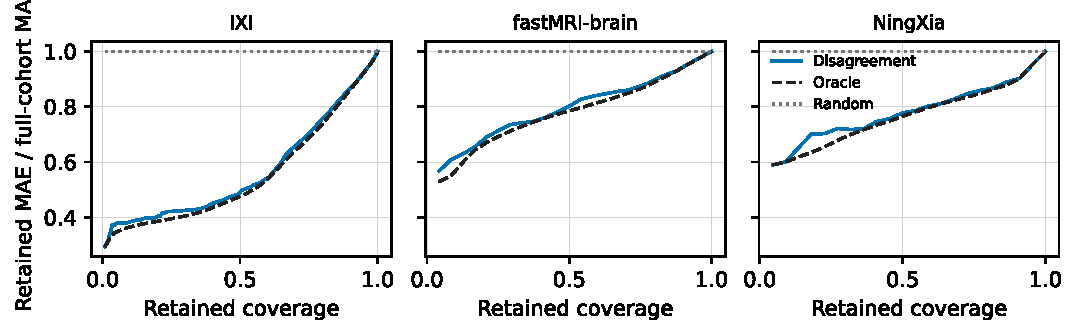
\includegraphics[width=0.82\textwidth]{figure_risk_coverage_outlined.pdf}
 \caption{Risk--coverage curves averaged over target interpolators after normalization by full-cohort MAE. The score remains between random and oracle review across cohorts; lower retained risk is better.}
 \label{fig:risk}
\end{figure*}

The complete curves in Fig.~\ref{fig:risk} avoid choosing a favorable test-set operating point. The largest absolute reduction occurs on IXI; smaller but consistent reductions occur on the two smaller cohorts. Because raw MAE is cohort-scale dependent, cross-cohort comparisons use nAURC and RRR rather than raw error.

\subsection{Registered selection and frozen transfer}
The model-bank audit found 11 neural and two analytical methods with complete, finite, affine- and shape-matched outputs on all fastMRI-brain/NingXia factors. I$^3$Net, HAT, and SwinIR are targets because they additionally exist on IXI; all other methods are peer candidates. Development evaluates 132 atomic score--mask--pooling candidates (74,052 case--target rows), then 40 promoted score--committee combinations spanning eight committee policies (22,440 rows). Selection uses IXI $\times4$ and fastMRI-brain $\times2/\times4/\times6$ only. Four roles are serialized before opening NingXia: the pre-specified method, development-selected universal and low-cost methods, and a shared/target decomposition.

\begin{table}[H]
 \centering
 \caption{Frozen finalists on development profiles. Metrics are equal-profile means; worst is maximum nAURC.}
 \resizebox{\columnwidth}{!}{\begin{tabular}{lcccc}
\toprule
Method & Mean nAURC & Worst & $\rho$ & RRR50 \\
\midrule
Pre-specified & 0.089 & 0.191 & 0.906 & 27.6\% \\
Low-cost & 0.087 & 0.159 & 0.906 & 27.8\% \\
Dev-selected universal & 0.040 & 0.099 & 0.947 & 28.1\% \\
Shared-difficulty & 0.036 & 0.093 & 0.952 & 28.1\% \\
\bottomrule
\end{tabular}
}
 \label{tab:dev}
\end{table}

The universal committee appears compelling on development (Table~\ref{tab:dev}), reducing mean/worst nAURC from 0.089/0.191 to 0.040/0.099. Its development-selected members are I$^3$Net, SAINT, SMamba-UNet, and Pix2PixGAN, with the named target removed when applicable. The decomposition selects weight one on target-invariant shared difficulty, a warning that examination severity rather than target attribution drives the development signal. Independent per-output normalization degrades rankings; a common source-intensity representation remains part of the scoring contract.

\subsection{Shared-error boundary and qualitative behavior}
The controlled stress test uses 20 fixed identity-sorted IXI examinations, all four targets, a foreground-constrained additive patch, five strengths, and a mask frozen before corruption. The target-specific arm perturbs only $\hat y_m$; the shared arm adds the identical patch to the target and every committee output.

\begin{figure}[H]
 \centering
 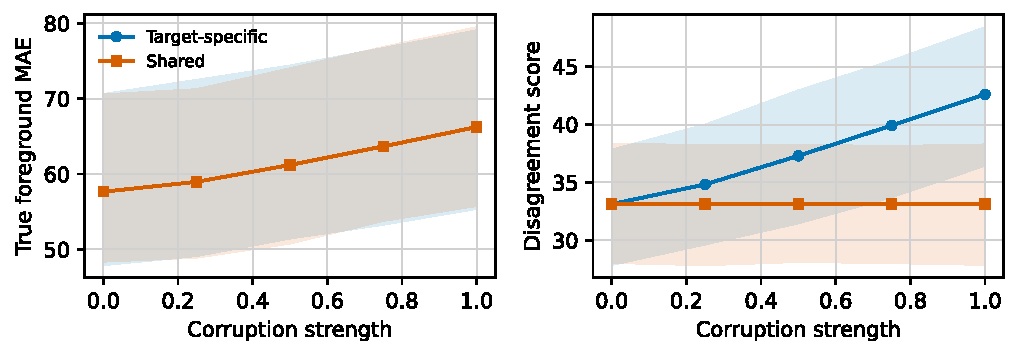
\includegraphics[width=0.98\columnwidth]{shared_error_stress_outlined.pdf}
 \caption{Controlled shared-error test. Target-specific corruption raises both MAE and disagreement; identical corruption of all outputs raises MAE while cancelling from target-to-member differences. Bands are 95\% bootstrap intervals.}
 \label{fig:stress}
\end{figure}

At maximum strength, target MAE rises by \StressMaeIncrease\ in both arms. Disagreement rises by \StressTargetIncrease\ for target-specific corruption but changes by \StressSharedChange\ under shared corruption, although mean committee MAE still rises by \StressCommitteeMaeIncrease. Figure~\ref{fig:stress} directly confirms Eq.~\eqref{eq:invariance}; it is an identifiability test rather than a simulation of all clinical failures.

\subsection{Independent-cohort validation and specificity}
\begin{table}[H]
 \centering
 \caption{One-shot NingXia OOF validation, averaged over three targets. No finalist was changed after validation.}
 \resizebox{\columnwidth}{!}{\begin{tabular}{llccc}
\toprule
Method & Factor & $\rho$ & nAURC$\downarrow$ & RRR50$\uparrow$ \\
\midrule
Pre-specified & $\times$2 & 0.903 & 0.059 & 22.3\% \\
\addlinespace[1.5pt]
Dev-selected universal & $\times$2 & 0.797 & 0.130 & 18.4\% \\
\addlinespace[1.5pt]
Low-cost & $\times$2 & 0.912 & 0.059 & 21.5\% \\
\addlinespace[1.5pt]
Shared-difficulty & $\times$2 & 0.859 & 0.098 & 19.5\% \\
\addlinespace[1.5pt]
Pre-specified & $\times$4 & 0.927 & 0.058 & 22.2\% \\
\addlinespace[1.5pt]
Dev-selected universal & $\times$4 & 0.906 & 0.062 & 22.2\% \\
\addlinespace[1.5pt]
Low-cost & $\times$4 & 0.922 & 0.055 & 22.2\% \\
\addlinespace[1.5pt]
Shared-difficulty & $\times$4 & 0.899 & 0.075 & 22.2\% \\
\addlinespace[1.5pt]
Pre-specified & $\times$6 & 0.874 & 0.094 & 20.9\% \\
\addlinespace[1.5pt]
Dev-selected universal & $\times$6 & 0.812 & 0.154 & 19.2\% \\
\addlinespace[1.5pt]
Low-cost & $\times$6 & 0.846 & 0.127 & 19.9\% \\
\addlinespace[1.5pt]
Shared-difficulty & $\times$6 & 0.784 & 0.160 & 19.4\% \\
\bottomrule
\end{tabular}
}
 \label{tab:validation}
\end{table}

\begin{figure*}[!t]
 \centering
 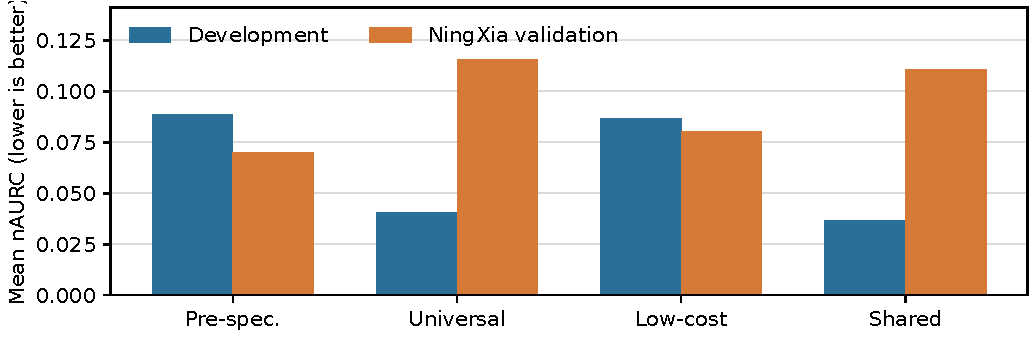
\includegraphics[width=0.80\textwidth]{figures_optimized/development_validation_transfer.pdf}
 \caption{Development selection does not transfer to frozen NingXia validation. Bars average fixed dataset--factor--target profiles; lower nAURC is better.}
 \label{fig:transfer}
\end{figure*}

The development gain reverses on validation (Table~\ref{tab:validation}, Fig.~\ref{fig:transfer}). The pre-specified method obtains mean/worst nAURC 0.070/0.125, $\rho=0.901$, and RRR50 21.8\%; the universal method obtains 0.116/0.207, 0.839, and 19.9\%. Its paired nAURC difference from baseline is +0.049 [95\% bootstrap interval $-0.038$, 0.244], so the data establish neither superiority nor uniform harm, but reject replacing the baseline. Low-cost scoring is closest (0.080, 0.893, 21.2\%) without a conclusive advantage.

Matched-target minus mismatched-target error correlation ranges from $-0.008$ to 0.014 on validation; intervals generally include zero. The score therefore ranks difficult examinations more reliably than it attributes failure to one target. Cross-factor voxel consistency is not reported: all 138 same-case comparisons have incompatible depth/generated support, and no post-validation resampling rule was introduced.

\subsection{Single-model comparison and measured cost}
On the same 24 fastMRI-brain $\times4$ SwinIR examinations, four-view TTA yields $\rho=0.960$ and nAURC 0.023 versus 0.931 and 0.061 for committee scoring. The paired nAURC difference is $-0.038$ [95\% CI $-0.119$, 0.001], so the apparent gain is not conclusive. Stored-output auditing takes 1.18 s mean/2.87 s p95 per examination on CPU with 0.89 GiB peak RSS; online use additionally incurs every neural reconstruction.

\section{Discussion and Conclusion}
The evidence supports examination triage more strongly than precise voxel localization. More importantly, the frozen transfer test shows that selecting committee members on reconstruction fidelity and development nAURC can overfit cohort-specific difficulty. A high $s_m$ prioritizes inspection while preserving reconstruction and committee identities; a low score indicates consensus only within that committee. Coverage should follow review capacity rather than a retrospectively tuned threshold.

The protocol is most attractive for retrospective audit, benchmark comparison, or systems that already cache several deterministic outputs. If only one model can be run, TTA, posterior sampling, acquisition residuals, or a validated error predictor may be more economical. A larger committee is not automatically better: member identity matters more than count, and the available no-reference diversity proxy cannot reliably choose the best compact subset. In practice, a review system should therefore freeze the committee specification, log member identities with every score, and monitor score distributions after software or acquisition changes rather than silently swapping members.

The score is also complementary to model-internal uncertainty. TTA probes sensitivity of one model to transformations, whereas cross-model disagreement probes separation from alternative reconstructions. Their failure modes need not coincide: one model may be unstable while peers agree, or all models may be confidently wrong together. A future deployment study should measure whether presenting both signals improves reviewer prioritization, review time, or downstream robustness without encouraging automation bias.

The principal limitations are structural. Shared errors are invisible, correlated members reduce diversity, a target mask can omit suppressed tissue, and unusual correct detail can be over-referred. Evidence remains restricted to T2 brain MRI; fastMRI-brain and NingXia are small, and matched analysis cannot separate target identity from shared difficulty. The universal-bank experiment tests stored outputs rather than uniform online latency; running all peers online is costly. There is no reader study or downstream task, and MAE is not diagnostic harm. Target-to-committee disagreement is therefore a reproducible selective-review ranking layer, not calibrated uncertainty, model attribution, or a clinical guarantee.

\clearpage
\bibliographystyle{IEEEbib}
\bibliography{references}
\end{document}
